\documentclass{article}

\usepackage{fancyhdr}
\usepackage{extramarks}
\usepackage{amsmath}
\usepackage{amsthm}
\usepackage{amsfonts}
\usepackage{tikz}
\usepackage[plain]{algorithm}
\usepackage{algpseudocode}
\usepackage{enumerate}
\usepackage{amssymb}
\usepackage{dsfont}
\usepackage{multicol}
\usepackage{graphicx}

\usetikzlibrary{automata,positioning,arrows}

\graphicspath{ {./images} }

%
% Basic Document Settings
%

\topmargin=-0.45in
\evensidemargin=0in
\oddsidemargin=0in
\textwidth=6.5in
\textheight=9.0in
\headsep=0.25in

\linespread{1.1}

\pagestyle{fancy}
\lhead{\hmwkAuthorName}
\chead{\hmwkClass:\ \hmwkTitle}
\rhead{\firstxmark}
\lfoot{\lastxmark}
\cfoot{\thepage}

\renewcommand\headrulewidth{0.4pt}
\renewcommand\footrulewidth{0.4pt}

\setlength\parindent{0pt}
\setlength{\parskip}{5pt}

%
% Create Problem Sections
%

\newcommand{\enterProblemHeader}[1]{ \nobreak\extramarks{}{Problem \arabic{#1} continued on next
    page\ldots}\nobreak{} \nobreak\extramarks{Problem \arabic{#1} (continued)}{Problem \arabic{#1}
    continued on next page\ldots}\nobreak{} }

\newcommand{\exitProblemHeader}[1]{ \nobreak\extramarks{Problem \arabic{#1} (continued)}{Problem
    \arabic{#1} continued on next page\ldots}\nobreak{}
    \stepcounter{#1}
    \nobreak\extramarks{Problem \arabic{#1}}{}\nobreak{}
}

\setcounter{secnumdepth}{0}
\newcounter{partCounter}
\newcounter{homeworkProblemCounter}
\setcounter{homeworkProblemCounter}{1}
\nobreak\extramarks{Problem \arabic{homeworkProblemCounter}}{}\nobreak{}

%
% Homework Problem Environment
%
% This environment takes an optional argument. When given, it will adjust the
% problem counter. This is useful for when the problems given for your
% assignment aren't sequential. See the last 3 problems of this template for an
% example.
%
\newenvironment{homeworkProblem}[1][-1]{
    \ifnum#1>0
        \setcounter{homeworkProblemCounter}{#1}
    \fi
    \section{Problem \arabic{homeworkProblemCounter}}
    \setcounter{partCounter}{1}
    \enterProblemHeader{homeworkProblemCounter}
}{
    \exitProblemHeader{homeworkProblemCounter}
}

%
% Homework Details
%   - Title
%   - Due date
%   - Class
%   - Section/Time
%   - Instructor
%   - Author
%

\newcommand{\hmwkTitle}{Homework\ \#5}
\newcommand{\hmwkDueDate}{May 24, 2024}
\newcommand{\hmwkClass}{MATH 188}
\newcommand{\hmwkClassInstructor}{Professor Kunnawalkam Elayavalli}
\newcommand{\hmwkAuthorName}{\textbf{Ray Tsai}}
\newcommand{\hmwkPID}{A16848188}

%
% Title Page
%

\title{
    \vspace{2in}
    \textmd{\textbf{\hmwkClass:\ \hmwkTitle}}\\
    \normalsize\vspace{0.1in}\small{Due\ on\ \hmwkDueDate\ at 23:59pm}\\
    \vspace{0.1in}\large{\textit{\hmwkClassInstructor}} \\
    \vspace{3in}
}

\author{
  \hmwkAuthorName \\
  \vspace{0.1in}\small\hmwkPID
}
\date{}

\renewcommand{\part}[1]{\textbf{\large Part \Alph{partCounter}}\stepcounter{partCounter}\\}

%
% Various Helper Commands
%

% Useful for algorithms
\newcommand{\alg}[1]{\textsc{\bfseries \footnotesize #1}}

% For derivatives
\newcommand{\deriv}[1]{\frac{\mathrm{d}}{\mathrm{d}x} (#1)}

% For partial derivatives
\newcommand{\pderiv}[2]{\frac{\partial}{\partial #1} (#2)}

% Integral dx
\newcommand{\dx}{\mathrm{d}x}

% Probability commands: Expectation, Variance, Covariance, Bias
\newcommand{\Var}{\mathrm{Var}}
\newcommand{\Cov}{\mathrm{Cov}}
\newcommand{\Bias}{\mathrm{Bias}}
\newcommand*{\Z}{\mathbb{Z}}
\newcommand*{\Q}{\mathbb{Q}}
\newcommand*{\R}{\mathbb{R}}
\newcommand*{\C}{\mathbb{C}}
\newcommand*{\N}{\mathbb{N}}
\newcommand*{\p}{\mathds{P}}
\newcommand*{\E}{\mathds{E}}

\begin{document}

\maketitle

\pagebreak

\begin{homeworkProblem}
  Let $B_n$ be the set of binary strings of length $n$, i.e., of words of length $n$ in the alphabet $\{0, 1\}$. Define a simple graph $H_n$ whose vertex set is $B_n$ and where two binary strings are connected by an edge if and only if they differ in exactly one position.

  Let $V$ be the real vector space with basis $\{v_x \mid x \in B_n\}$. It's not convenient to pick an ordering of the vertices to write down the adjacency matrix. Instead, we will think of the adjacency matrix $A$ of $H_n$ as a linear operator on $V$:
  \[
    A \sum_{x \in B_n} c_x v_x = \sum_{x \in B_n} c_x \sum_{\substack{y \text{ such that} \\ \{y,x\} \text{ is an edge}}} v_y.
  \]
  \begin{enumerate}[(a)]
    \item For each $x \in B_n$, define $E_x \in V$ by
    \[
      E_x = \sum_{y \in B_n} (-1)^{x \cdot y} v_y,
    \]
    where $x \cdot y = x_1y_1 + \ldots + x_ny_n$. Show that this is an eigenvector for $A$ with eigenvalue $n - 2|x|$ where $|x|$ is the number of $x_i$ equal to 1.

    \begin{proof}
      Let $x \in B_n$. Let $N(x)$ denote the set of neighbors of $x$ in $H_n$, and let $x_i$ denote the $i$th digit of $x$. We first note that
      \[
        E_x = \sum_{\substack{y \in B_n \\ x \cdot y \text{ is even}}} v_y - \sum_{\substack{y \in B_n \\ x \cdot y \text{ is odd}}} v_y
      \]
      Hence, we may write
      \begin{align}
        AE_x
        &= A\sum_{\substack{y \in B_n \\ x \cdot y \text{ is even}}} v_y - A\sum_{\substack{y \in B_n \\ x \cdot y \text{ is odd}}} v_y \\
        &= \sum_{\substack{y \in B_n \\ x \cdot y \text{ is even}}} \sum_{y' \in N(y)} v_{y'} - \sum_{\substack{y \in B_n \\ x \cdot y \text{ is odd}}} \sum_{y' \in N(y)} v_{y'} \\
        &=  \sum_{\substack{y \in B_n \\ x \cdot y \text{ is even}}} \left(\sum_{\substack{y' \in N(y) \\ x \cdot y' \text{ is even}}} v_{y'} + \sum_{\substack{y' \in N(y) \\ x \cdot y' \text{ is odd}}} v_{y'}\right) - \sum_{\substack{y \in B_n \\ x \cdot y \text{ is odd}}} \left(\sum_{\substack{y' \in N(y) \\ x \cdot y' \text{ is even}}} v_{y'} + \sum_{\substack{y' \in N(z) \\ x \cdot y' \text{ is odd}}} v_{y'}\right).
      \end{align}
      Given a $y' \in B_n$. Let $y \in N(y')$ such that $y_i \neq y'_i$. Suppose $x \cdot y'$ is even. Notice that $x \cdot y$ remains even if and only if $x_i = 0$. Similarly, when $x \cdot y'$ is odd, $x \cdot y$ remains odd if and only if $x_i = 0$. 
      
      Hence, $y'$ has $n - |x|$ number of neighbors $y$ such that $x \cdot y' \equiv x \cdot y \pmod 2$ and $|x|$ number of neighbors $y$ such that $x \cdot y' \not\equiv x \cdot y \pmod 2$

      But then for all $y' \in B_n$, (3) adds $v_{y'}$ $(n - 2|x|)$ times if $x \cdot y'$ is even and adds $-v_{y'}$ $(n - 2|x|)$ times if if $x \cdot y'$ is odd. It now follows that
      \[
        AE_x = (n - 2|x|)\left(\sum_{\substack{y \in B_n \\ x \cdot y \text{ is even}}} v_y - \sum_{\substack{y \in B_n \\ x \cdot y \text{ is odd}}} v_y\right) = (n - 2|x|)E_x.
      \]
    \end{proof}

    \newpage
    
    \item For $x \in B_n$ and a non-negative integer $d$, give a formula for the number of closed walks of length $d$ in $H_n$ beginning at $x$. [You may assume without proof that $\{E_x \mid x \in B_n\}$ is linearly independent.]

    \begin{proof}
      Let $x, y \in B_n$. We first show that
      \begin{gather}
        \# \text{closed walks of } x \text{ of length }d = \# \text{closed walks of } y \text{ of length }d.
      \end{gather}
      Suppose $x$ and $y$ differ at positions $i_1, i_2, \dots, i_N$. Let $W$ be a length-$d$ closed walk of $x$, say $w_1w_2 \ldots w_d$. For each $w_i$ in $W$, we flip $w$'s $i_k$th digit, for $i \leq k \leq N$. Let $W'$ be the resulting sequence of strings. Obviously, $w_1' = w_d' = y$. Since we flip the same positions of each string in $W$, the operation above perserves the difference of positions between each string. That is, for each consecutive strings $w_i'$ and $w_{i + 1}'$ in $W'$, $w_i'$ and $w_{i + 1}'$ differ at only 1 position. Hence, $\{w_i', w_{i + 1}'\}$ is an edge in $H_n$. But then $W'$ is a closed walk of $y$ of length $d$. Note that applying the operation again on $W'$ yields $W$, and thus the equality of (4). 
      
      But then (4) also implies that the number of closed walks of length $d$ beginning at any vertex is the same. By Proposition 4.6, the number of closed walks in $H_n$ of length 
      \[
        tr(A^d) = \sum_{x \in B_n} (n - 2|x|)^d = \sum_{i = 0}^n \binom{n}{i}(n - 2i)^d
      \]
      Hence,
      \[
        \# \text{closed walks of } x \text{ of length }d = 2^{-n}\sum_{i = 0}^n \binom{n}{i}(n - 2i)^d
      \]
    \end{proof}
  \end{enumerate}
\end{homeworkProblem}

\newpage

\begin{homeworkProblem}
  \begin{enumerate}[(a)]
    \item Fix a positive integer $k$. Construct a directed graph for which walks (between certain vertices) can be interpreted as binary strings with exactly $k$ zeroes. Explain clearly how this interpretation works, including how the length of the walk relates to the length of the binary string.
    \begin{proof}
      Consider a directed graph $G$ where the vertex set $V = [k + 1]$ and the edge set
      \[
        E = \{(i, j) : j \geq i \text{ and } i, j \in [k + 1]\}.
      \]
      We show that 
      \[
        \# \text{binary strings with exactly } k \text{ zeros and } n + 1 \text{ ones} = \# \text{walks on } G \text{ of length $n$}.
      \]
      Given a binary strings $S$ with exactly $k$ zeros and $n + 1$ ones, we may construct an increase sequence $W$ of integers in $[k + 1]$, where the number of $i$'s in $W$ is the number of 1's between the after the $(i - 1)$th 0 or before the $i$th 0 of $S$ (they are the same unless $i = 1$ or $k + 1$). Since $W$ is increasing, each consecutive pair of numbers in $W$ corresponds to precisely one edge in $G$, and thus $W$ is a well-defined walk on $G$. Since $W$ is a sequence of length $n + 1$, it corresponds to a walk of length $n$.
      
      Now suppose we have a walk $W'$ of length $n$ on $G$. We may consider $W'$ as a increasing sequence with length $n + 1$ of integers in $[k + 1]$. Since $W'$ is an increasing sequence, there is a unique binary string $S'$ with $k$ zeros and $n + 1$ ones, where the number of 1's after the $(i - 1)$th 0 or before the $i$th 0 of $S$ is the number of $i$'s in $W$. 
      
      Since the two described operations are inverses of each other, the equality above holds, and a walk of length $n$ corresponds to a binary string of length $n + k + 1$.
    \end{proof}
    \item Construct a directed graph for which walks (between certain vertices) can be interpreted as binary strings in which no symbol ever appears 3 times in a row. Explain clearly how this interpretation works, including how the length of the walk relates to the length of the binary string.
    \begin{proof}
      Consider the following graph $G$:
      \begin{center}
        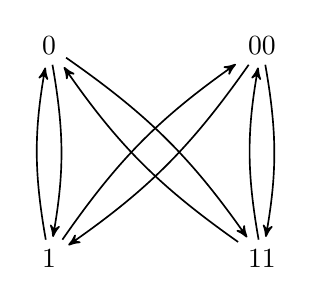
\begin{tikzpicture}[->,>=stealth',shorten >=1pt, auto, node distance=2cm, semithick]

        \node (A)          {$0$}; \node (B) [below of=A, yshift=-20pt] {$1$}; \node (A') [right of=A, xshift=20pt] {$00$}; \node (B') [below of=A', yshift=-20pt] {$11$};
      
        \path (A) edge [left=20, above, bend left=10] node {} (B) (B) edge [left=20, above, bend left=10] node {} (A) (A') edge [left=20, above, bend left=10] node {} (B) (B) edge [left=20, above, bend left=10] node {} (A') (B') edge [left=20, above, bend left=10] node {} (A) (A) edge [left=20, above, bend left=10] node {} (B') (A') edge [left=20, above, bend left=10] node {} (B') (B') edge [left=20, above, bend left=10] node {} (A') ;
        \end{tikzpicture}
      \end{center}
      We show that 
      \[
        \# \text{binary strings without $000$ and $111$} = \# \text{walks on } G.
      \]
      Suppose we have a binary string $S$ without $000$ and $111$, say $s_1s_2 \ldots s_n$. We inductively construct a walk $W = w_1w_2, \dots w_m$ on $G$ in the following way: Put $w_1 = s_1$. Suppose we obtain a walk $W' = w_1\ldots w_l$ after going through $s_1, \dots, s_{k - 1}$, for some $k \geq 2$. If $w_l = s_k$, replace $w_l$ with the vertex $s_ks_k$. Notice that since $S$ does not contain $s_ks_ks_k$, $w_{l - 1} \neq s_k$ in this case, as thus $(w_{l - 1}, w_l)$ is an edge in $G$. Otherwise, of $w_l \neq s_k$, append a new vertex $w_{l + 1} = s_k$ to $W$, and obviously $(w_{l}, w_{l + 1})$ is an edge in $G$. Since each choice of edge in the inductive step is unique and valid, $W$ is a well-defined walk on $G$. In each inductive step $k$, we only extend the length of $W$ by one when $s_k \neq s_{k - 1}$, and thus $W$ contains $n - r$ vertices, where $r$ is the number of $00$ and $11$ in $S$. 

      Now suppose we have a walk $X$ with $n - r$ vertices on $G$, where $r$ is the number of $00$ and $11$'s in $X$. We may convert $X$ to a binary string $T$ by concatenating the corresponding of each vertex in $X$. Since $X$ does not contain edges $(0, 00), (00, 0), (1, 11), (11, 1)$, $T$ is unique and does not contain $000$ and $111$, and thus $T$ is well defined. Since $X$ contains $r$ number of vertices $00$ and $11$'s, $T$ has length $(n - r) + r = n$.

      The two described operations are obvisouly inverses of each other, so the equality holds and a walk of length $n - r - 1$ corresponds to a binary string of length $n$ without $000$ and $111$.
    \end{proof}
  \end{enumerate}
\end{homeworkProblem}

\newpage

\begin{homeworkProblem}
  \begin{enumerate}[(a)]
    \item We have $n$ distinguishable tables. We want to paint each one either red, blue, or green such that an odd number of them are red and an even number of them are blue. How many ways can this be done?
    \begin{proof}
      Suppose $S$ is a set of tables. Let $\alpha(S)$ be the set of ways to paint the tables red according to our rules, so $|\alpha(S)| = 1$ if $|S|$ is odd and $|\alpha(S)| = 0$ otherwise. Similarly, let $|\beta(S)|$ be the set of ways to paint the table blue according to our rules, so $|\beta(S)| = 1$ if $|S|$ is even and $|\beta(S)| = 0$ otherwise. Finally, let $\gamma(S)$ be the set of ways to paint the table green according to our rules, so $|\gamma(S)| = 1$. Hence, 
      \[
        E_{\gamma}(x) = \sum_{n \geq 0} \frac{x^n}{n!} = e^x.
      \]
      \[
        E_{\beta}(x) = \sum_{n \geq 0} \frac{x^{2n}}{(2n)!} = (e^x + e^{-x})/2.
      \]
      \[
        E_{\alpha}(x) = \sum_{n \geq 0} \frac{x^{2n + 1}}{(2n + 1)!} = e^x - \sum_{n \geq 0} \frac{x^{2n}}{(2n)!} = (e^x - e^{-x})/2.
      \]
      It now follows that
      \[
        E_{\alpha \cdot \beta \cdot \gamma}(x) = E_{\alpha}E_{\beta}E_{\gamma}(x) = \frac{1}{4}e^x(e^x + e^{-x})(e^x - e^{-x}) = \frac{1}{4}(e^{3x} - e^{-x}) = \frac{1}{4}\sum_{n \geq 0} \frac{(3^n - (-1)^n)x^n}{n!}.
      \]
      Hence, there are
      \[
        n![x^n]E_{\alpha \cdot \beta \cdot \gamma}(x) = \frac{(3^n + (-1)^{n + 1})}{4}
      \]
      ways to color the the $n$ tables.
    \end{proof}
    \item Continuing with (a), we add the colors white and yellow, but the total number of tables which are white or yellow must be even (in symbols: \#white tables + \#yellow tables is even). How many ways are there to choose colors?
    \begin{proof}
      Let $\delta(S)$ be the set of ways to paint the tables either white or yellow according to our rules, so $|\delta(S)| = 2^{|S|}$ if $|S|$ is even and $|\delta(S)| = 0$ otherwise. Hence,
      \[
        E_{\delta}(x) = \sum_{n \geq 0} \frac{(2x)^{2n}}{(2n)!} = (e^{2x} + e^{-2x})/2.
      \]
      It now follows that
      \begin{align*}
        E_{\alpha \cdot \beta \cdot \gamma \cdot \delta}(x) 
        &= E_{\alpha \cdot \beta \cdot \gamma}(x)E_{\delta}(x) \\ 
        &= \frac{1}{8}(e^{3x} - e^{-x})(e^{2x} + e^{-2x}) \\
        &= \frac{1}{8}(e^{5x} - e^{-3x}) = \frac{1}{8}\sum_{n \geq 0} \frac{(5^n - (-3)^n)x^n}{n!}.
      \end{align*}
      Hence, there are
      \[
        n![x^n]E_{\alpha \cdot \beta \cdot \gamma \cdot \delta}(x) = \frac{5^n - (-3)^n}{8}
      \]
      ways to color $n$ tables with our rules.
    \end{proof}
  \end{enumerate}
\end{homeworkProblem}

\newpage

\begin{homeworkProblem}
  Let $b_{n,k}$ be the number of set partitions of $[n]$ with $k$ blocks such that every block has an even (and positive) number of elements and let $b_n$ be the same, but with no restriction on the number of blocks.
\begin{enumerate}[(a)]
    \item Find a formula for the EGF $B_k(x) = \sum_{n \geq 0} b_{n,k} \frac{x^n}{n!}$.
    \begin{proof}
      Consider the selection structure
      \[
        \beta(S) = \begin{cases}
          \{1\} & \text{if } |S| > 0 \text{ and } |S| \text{ is even} \\
          \emptyset & \text{otherwise}
        \end{cases},
      \]
      which picks out nonempty subsets of even size. But then, $\beta^k(S)$ is the set of ordered set partitions of $S$ with $k$ blocks of even sizes. Hence,
      \[
        \sum_{n \geq 0} k!b_{n, k}\frac{x^n}{n!} = E_{\beta^k}(x) = E_{\beta}(x)^k = \left(\frac{e^x + e^{-x}}{2} - 1\right)^k,
      \]
      and thus
      \[
        B_k(x) = \sum_{n \geq 0} b_{n, k}\frac{x^n}{n!} = \frac{(e^x + e^{-x} - 2)^k}{2^kk!}
      \]
    \end{proof}
    \item Find a formula for the EGF $B(x) = \sum_{n \geq 0} b_n \frac{x^n}{n!}$.
    \begin{proof}
      We continue using the selection structure $\beta$ from (a). Then, $e^{\beta}(S)$ can be interpreted as the set of partitions of $[n]$ such that all blocks are of even sizes. It now follows that
      \[
        B(x) = E_{e^{\beta}}(x) = \exp(E_{\beta}(x)) = \exp\left(\frac{e^x + e^{-x}}{2} - 1\right).
      \]
    \end{proof}
\end{enumerate}
\end{homeworkProblem}

\newpage

\begin{homeworkProblem}
  Let $a_n$ be the number of functions $f: [n] \rightarrow [n]$ such that $f \circ f = f$. Find a simple formula for the EGF $A(x) = \sum_{n \geq 0} a_n \frac{x^n}{n!}$.

  \begin{proof}
    For each $f: [n] \to [n]$, we associate a directed graph $G_f$ with vertex set $[n]$ and edge set $\{(i, j) : f(i) = j\}$. Suppose $f \circ f = f$. Say we have $i, j \in [n]$ such that $f(i) = j$. Then, $f(j) = f(f(i)) = f(i) = j$. That is, any vertex with an incoming edge cannot have an outgoing edge to another vertex. Hence, given a component $C \subseteq G_f$ of size $n$, $C$ is of the form of a star, where all vertex points in the component point to a $sink$ vertex. Since there are $n$ vertices in $C$, there are $n$ ways to pick the $sink$ vertex, and thus $C$ has $n$ possible configurations. This allows us to define structure $\alpha(S) = |S|$, which picks out the components that could be in $G_f$, with each element in $\alpha(S)$ being the $sink$ vertex of a component of size $|S|$. Then, $e^{\alpha}([n])$ can be interpreted as the set of possible graphs $G_f$, where $f: [n] \to [n]$ such that $f \circ f = f$. Thus, $e^{\alpha}([n])$ is also interpreted as the set of $f: [n]
    \to [n]$ such that $f \circ f = f$. It now follows that
    \[
      A(x) = E_{e^{\alpha}}(x) = \exp(E_{\alpha}(x)) = \exp\left(\sum_{n \geq 1} \frac{x^n}{(n - 1)!}\right) = e^{xe^x}.
    \]
  \end{proof}
\end{homeworkProblem}

\newpage

\begin{homeworkProblem}
  Explain why it is impossible to have a directed graph for which walks of length $2n$ can be interpreted as balanced sets of $n$ pairs of parentheses.

  \begin{proof}
    Suppose not. We have a graph $G$ for which the number of walks of length $2n$ equals to $C_n$, the $n$th Catalan number. Let $A$ be the transition matrix of $G$. The number of length $2n$ walks on $G$ is the sum of all entries of $A^{2n}$. Hence, the generating function for walks of even length is 
    \[
      W(x) = \sum_{k \geq 0} \sum_{i, j} (A^{2k})_{i, j}x^k = \sum_{i, j} F_{A^2; i, j}(x).
    \]
    By Theorem 4.9, $F_{A^2; i, j}(x)$ is a rational generating function, which makes $W(x)$ also rational. But then by Remark 2.30, $C(x) = \sum_{n \geq 0} C_nx^n$ is not a rational generating function, contradiction.
  \end{proof}
\end{homeworkProblem}

\newpage

\begin{homeworkProblem}
  Let $A$ be the adjacency matrix of the following directed graph:
  \begin{center}
    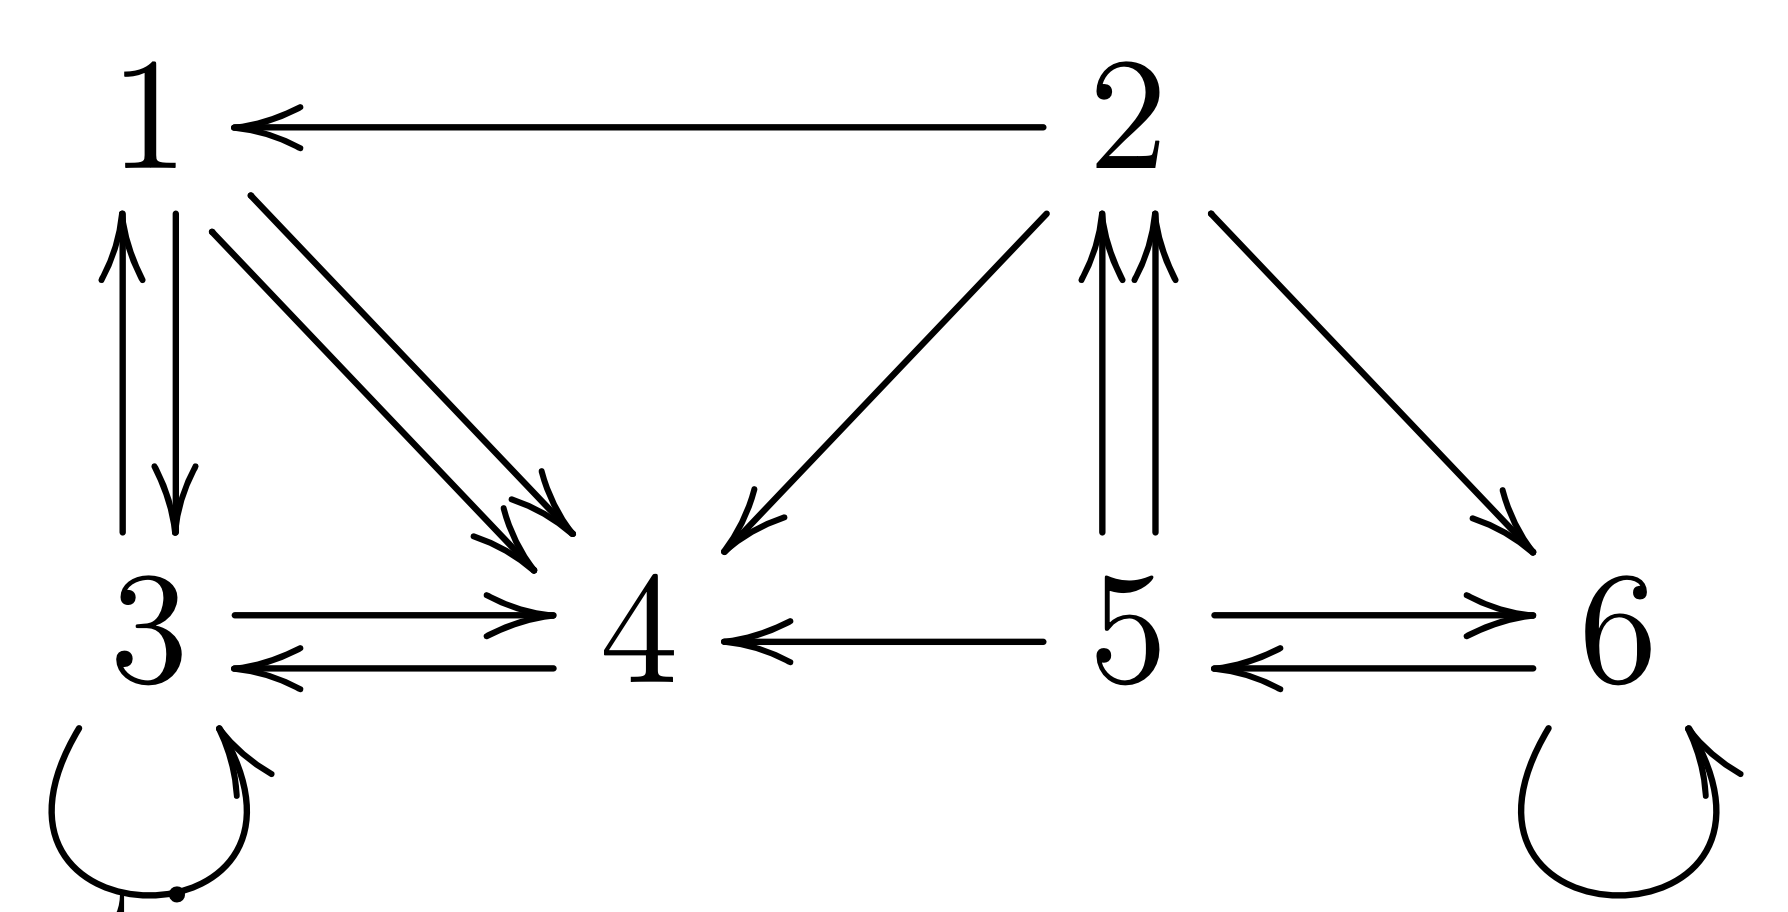
\includegraphics[width=0.3\textwidth]{Q7}
  \end{center}
  Express $F_{A;1,4}(x)$ as a rational function.

  \begin{proof}
    We first note that
    \[
      A = \begin{bmatrix}
        0 & 0 & 1 & 2 & 0 & 0 \\
        1 & 0 & 0 & 1 & 0 & 1 \\
        1 & 0 & 1 & 1 & 0 & 0 \\
        0 & 0 & 1 & 0 & 0 & 0 \\
        0 & 2 & 0 & 1 & 0 & 1 \\
        0 & 0 & 0 & 0 & 1 & 1 \\
      \end{bmatrix}.
    \]
    By Theorem 4.9, we have
    \[
      F_{A;1,4}(x) = -\frac{\det((I_6 - xA); 4, 1)}{\det(I_6 - xA)}.
    \]
    By MATLAB,
    \[
      \det(I_6 - xA) = 4x^6 + 6x^5 + 6x^4 - x^3 - 2x^2 - 2x + 1,
    \]
    \[
      \det((I_6 - xA); 4, 1) = x(-2x^4 + 3x^3 + x^2 + 3x - 2).
    \]
    Hence,
    \[
      F_{A;1,4}(x) = -\frac{x(-2x^4 + 3x^3 + x^2 + 3x - 2)}{4x^6 + 6x^5 + 6x^4 - x^3 - 2x^2 - 2x + 1} = \frac{x(x-2)}{2x^3 + 2x^2 + x - 1}.
    \]
  \end{proof}
\end{homeworkProblem}

\newpage

\begin{homeworkProblem}
  Compute $G_3$ in Example 4.11.

  \begin{proof}
    Here is $G_3$:
    \begin{center}
      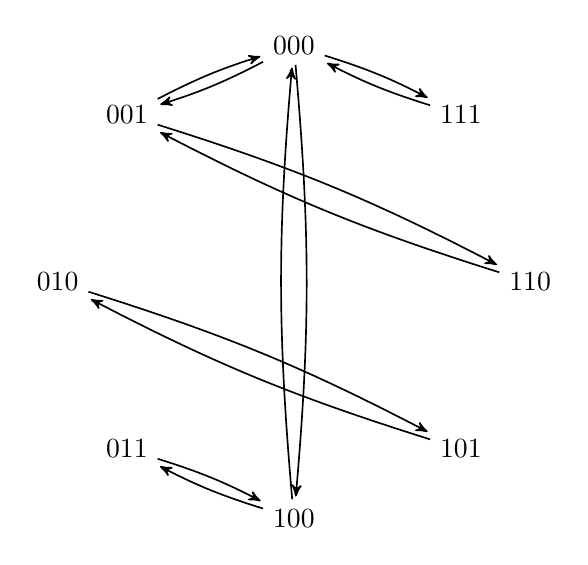
\begin{tikzpicture}[->,>=stealth',shorten >=1pt, auto, node distance=1cm, semithick]
        \def\n{8}

        \def\c{5}
    
        \def\radius{3}
    
        \node (v0) at ({2*360/\n}:\radius) {$000$}; \node (v1) at ({3*360/\n}:\radius) {$001$}; \node (v2) at ({4*360/\n}:\radius) {$010$}; \node (v3) at ({5*360/\n}:\radius) {$011$}; \node (v4) at ({6*360/\n}:\radius) {$100$}; \node (v5) at ({7*360/\n}:\radius) {$101$}; \node (v6) at ({8*360/\n}:\radius) {$110$}; \node (v7) at ({1*360/\n}:\radius) {$111$};

        \path (v0) edge [bend left=\c] node {} (v1) (v0) edge [bend left=\c] node {} (v4) (v0) edge [bend left=\c] node {} (v7)

              (v1) edge [bend left=\c] node {} (v0) (v1) edge [bend left=\c] node {} (v6)

              (v2) edge [bend left=\c] node {} (v5)

              (v3) edge [bend left=\c] node {} (v4)

              (v4) edge [bend left=\c] node {} (v0) (v4) edge [bend left=\c] node {} (v3)

              (v5) edge [bend left=\c] node {} (v2)

              (v6) edge [bend left=\c] node {} (v1)

              (v7) edge [bend left=\c] node {} (v0) ;
      \end{tikzpicture}
    \end{center}
  \end{proof}
\end{homeworkProblem}

\newpage

\begin{homeworkProblem}
  Given a sequence $(a_n)_{n \geq 0}$ we define its $q$-EGF to be
  \[
    A(x) = \sum_{n \geq 0} a_n \frac{x^n}{[n]_q!}.
  \]
  What is the $q$-analogue of Proposition 5.2?

  \begin{proof}
    Suppose we have $A(x) = \sum_{n \geq 0} a_n \frac{x^n}{[n]_q!}$ and $B(x) = \sum_{n \geq 0} b_n \frac{x^n}{[n]_q!}$. Then,
    \begin{gather}
      A(x) + B(x) = \sum_{n \geq 0} (a_n + b_n)\frac{x^n}{[n]_q!} \\
      A(x)B(x) = \sum_{n \geq 0} \sum_{i = 0}^n \frac{a_i}{[i]_q!}\frac{b_{n - i}}{[n - i]_q!}x^n = \sum_{n \geq 0} \left(\sum_{i = 0}^n \begin{bmatrix}
        n \\
        i
      \end{bmatrix}_q a_ib_{n - 1}\right) \frac{x^n}{[n]_q!}.
    \end{gather}
    Define $q$-structure $\alpha_q$, which takes as input a finite vector space $V$ of $\textbf{F}_q$ and outputs a finite vector space $\alpha_q(V)$, with the property that $\dim \alpha_q(V) = \dim \alpha_q(U)$ whenever $\dim V = \dim U$. Let $\alpha_q, \beta_q$ be $q$-structures. Define the addition and multiplication of $q$-structures to be
    \begin{gather*}
      (\alpha_q + \beta_q)(V) = \alpha_q(V) \oplus \beta_q(V) \\
      (\alpha_q \cdot \beta_q)(V) = \bigoplus_{S \text{ subspace of } V} \alpha_q(S) \otimes \beta_q(S^{\bot}). 
    \end{gather*}
    Define the $q$-EGF associated to structure $\alpha_q$ to be
    \[
      E_{q_{\alpha}}(x) = \sum_{n \geq 0} \dim \alpha_q(\textbf{F}_q^n) \frac{x^n}{[n]_q!}.
    \]
    We show that
    \[
      E_{\alpha_q + \beta_q}(x) = E_{\alpha_q}(x) + E_{\beta_q}(x), \quad E_{\alpha_q \cdot \beta_q}(x) = E_{\alpha_q}(x)E_{\beta_q}(x).
    \]
    For the sum, we have $\dim (\alpha_q + \beta_q)(\textbf{F}_q^n) = \dim \alpha_q(\textbf{F}_q^n) + \dim \beta_q(\textbf{F}_q^n)$, which is the coefficient of $E_{\alpha_q}(x) + E_{\beta_q}(x)$ by (5). On the other hand , we have 
    \[
      |(\alpha_q \cdot \beta_q)(\textbf{F}_q^n)| = \sum_{S \text{ subspace of } \textbf{F}_q^n} \dim \alpha_q(S) \cdot \dim \beta_q(S^{\bot}) = \sum_{i = 0}^n \begin{bmatrix}
        n \\
        i
      \end{bmatrix}_q \dim \alpha_q(\textbf{F}_q^i) \cdot \dim \beta_q(\textbf{F}_q^{n - i}).
    \]
    for the product, which is the coefficient of $E_{\alpha_q}(x)E_{\beta_q}(x)$ by (6).
  \end{proof}
\end{homeworkProblem}

\newpage

\begin{homeworkProblem}
  Let $n$ be a positive integer. Given a group of $n$ people, we want to divide them into nonempty committees and choose a leader for each committee, and also choose one of the committees to be in charge of all the others. Let $h_n$ be the number of ways to do this and set $h_0 = 1$. Give a simple expression for the exponential generating function $H(x) = \sum_{n \geq 0} h_n \frac{x^n}{n!}$.

  \begin{proof}
    Define 
    \[
      \alpha(S) = S
    \]
    which outputs the ways to pick an element from the input set $S$. Hence, if $S$ is the set of committee members, $\alpha(S)$ is the set of ways to select a leader from $S$. On the other hand, if $S$ is the set of committees, $\alpha(S)$ is the set of ways to choose a leading committee. 

    According to our rules, for each partition of $n$ people, we apply the $\alpha$ structure to each block of people to choose a leader, then we apply $\alpha$ to the partition as a whole to choose the leading committee. But then this is just $\alpha \circ \alpha([n])$, and so $H(x) = E_{\alpha \circ \alpha}$. Since
    \[
      E_{\alpha}(x) = \sum_{n \geq 0} \frac{nx^n}{n!} = \sum_{n \geq 1} \frac{x^n}{(n - 1)!} = xe^x,
    \]
    it now follows that
    \[
      H(x) = E_{\alpha \circ \alpha} = E_{\alpha}\left(xe^x\right) = xe^xe^{xe^x} = xe^{x(1 + e^x)}.
    \]
  \end{proof}
\end{homeworkProblem}

\newpage

\begin{homeworkProblem}
  Let $h_n$ be the number of bijections $f: [n] \rightarrow [n]$ with the property that $f \circ f \circ f$ is the identity function. Give a simple expression for the exponential generating function $H(x) = \sum_{n \geq 0} h_n \frac{x^n}{n!}$.

  \begin{proof}
    Suppose bijection $f: [n] \rightarrow [n]$ has the property that $f \circ f \circ f$ is the identity function. Then, $f$ is a permutation on $[n]$ whose cycles all have length $1$ or $3$. Let $\alpha(S)$ be the set of cyclic orderings of $S$ if $|S| = 1 \text{ or } 3$ and $\alpha(S) = \emptyset$ otherwise. Then, $E_{\alpha} = x + \frac{x^3}{3}$. But then $e^{\alpha}$ can be interpreted as the set of bijections $f$ with $f \circ f \circ f$ being the identity. It now follows that
    \[
      E_{e^{\alpha}}(x) = \exp\left(x + \frac{x^3}{3}\right).
    \]
  \end{proof}
\end{homeworkProblem}

\newpage

\begin{homeworkProblem}
  Given $G(x)$ with $G(0) \neq 0$, define its \textit{logarithmic derivative} to be $\mathcal{L}(G) = \frac{DG(x)}{G(x)}$.
  \begin{enumerate}[(a)]
    \item Show that for any $F(x)$, we have $\mathcal{L}(\exp(F(x))) = DF(x)$.
    \begin{proof}
      We first note that
      \[
        D\exp(F(x)) = DF(x)\sum_{n \geq 1} \frac{(F(x))^{n - 1}}{(n - 1)!} = (DF(x))\exp(F(x)).
      \]
      Hence,
      \[
        \mathcal{L}(\exp(F(x))) = \frac{D\exp(F(x))}{\exp(F(x))} = \frac{(DF(x))\exp(F(x))}{\exp(F(x))} = DF(x).
      \]
    \end{proof}
    \item Show that if $G_1(0) = G_2(0) = 0$, then $\mathcal{L}(G_1(x)G_2(x)) = \mathcal{L}(G_1(x)) + \mathcal{L}(G_2(x))$.
    \begin{proof}
      \begin{align*}
        \mathcal{L}(G_1(x)G_2(x))
        &= \frac{D(G_1(x)G_2(x))}{G_1(x)G_2(x)} \\
        &= \frac{G_2(x)DG_1(x) + G_1(x)DG_2(x)}{G_1(x)G_2(x)} \\
        &= \frac{DG_1(x)}{G_1(x)} + \frac{DG_2(x)}{G_2(x)} = \mathcal{L}(G_1(x)) + \mathcal{L}(G_2(x)).
      \end{align*}
    \end{proof}
    \item Let $a_n$ be the number of involutions of size $n$ and let $A(x) = \sum_{n \geq 0} a_n \frac{x^n}{n!}$. From Example 5.11, we have $A(x) = \exp(x + \frac{x^2}{2})$. Apply $\mathcal{L}$ to prove for all $n \geq 0$ that $a_{n+2} = a_{n+1} + (n + 1)a_n$.
    \begin{proof}
      By (a) and (b),
      \[
        \frac{DA(x)}{A(x)} = \mathcal{L}(A(x)) = \mathcal{L}(e^xe^{x^2/2}) = \mathcal{L}(e^x) + \mathcal{L}(e^{x^2/2}) = Dx + D\left(\frac{x^2}{2}\right) = 1 + x.
      \]
      Hence,
      \[
        D(A(x)) = (1 + x)A(x).
      \]
      Since
      \[
        D(A(x)) = \sum_{n \geq 1} a_n \frac{x^{n - 1}}{(n - 1)!} = \sum_{n \geq 0} a_{n + 1} \frac{x^n}{n!},
      \]
      \begin{align*}
        (1 + x)A(x) 
        &= \sum_{n \geq 0}a_n\frac{x^n}{n!} + \sum_{n \geq 0}a_n\frac{x^{n + 1}}{n!} \\
        &= a_0 + \sum_{n \geq 0}a_n\frac{x^n}{n!} + \sum_{n \geq 1}a_{n - 1}\frac{x^{n}}{(n - 1)!},
      \end{align*}
      for all $n \geq 1$,
      \[
        a_{n + 1} = a_n + na_{n - 1},
      \]
      and the result now follows.
    \end{proof}
  \end{enumerate}
\end{homeworkProblem}
\end{document}